\chapter[Forschungsfrage 3]{Welche besonderen sicherheitstechnischen Aspekte muss ein solcher Prozess im Bereich der Versicherung erfüllen?} \label{ff3}
Diese Kapitel ... <Einführung ins Kapitel>
\par
Informations- und Kommunikationssysteme sind in der heutigen Gesellschaft von elementarer Bedeutung -- sie spielen eine immer größer werdende Rolle. Der Innovationsgrad in der Informationstechnik ist konstant hoch und deswegen sind folgende Bereiche ständiger Weiterentwicklung unterlegen: steigende Vernetzung der Bevölkerung, IT-Verbreitung und Durchdringung, verschwinden der Netzgrenzen, kürze Angriffszyklen auf wichtige Infrastruktur, höhere Interaktivität von Anwendungen und die Verantwortung der Benutzer eines IT-Systems.\autocite[vgl.][S.\,2f.]{bundesamt_fur_sicherheit_in_der_informationstechnik_bsi_it-grundschutz-kompendium_2020}

\section{Grundlagen: Sicherheitstechnische Anforderungen}\label{kap:sicherheitstechnischeAnforderungen}
Informationen sind elementarer Bestandteil der heutigen Welt -- diese sind von sehr hohem Wert für Unternehmen, Behörden und Privatpersonen. Die meisten Geschäftsprozesse, die im heutigen Prozessablauf einer Organisation verankert sind, funktionieren nicht ohne IT-Unterstützung. Somit ist die Informationstechnologie zentraler Bestandteil jedes Unternehmens. Deswegen ist ein zuverlässiges System mit entsprechender Soft- und Hardware unerlässlich. Es muss darauf geachtet werden, dass die Informationen, die auf diesem System verteilt sind, ausreichend gut geschützt sind, damit es nicht zu einer Bedrohungslage kommt. Unzureichend geschützte Systeme stellen ein sehr hohes Risiko dar. \enquote{Dabei ist ein vernünftiger Informationsschutz ebenso wie eine Grundsicherung der IT schon mit verhältnismäßig geringen Mitteln zu erreichen. Die verarbeiteten Daten und Informationen müssen adäquat geschützt, Sicherheitsmaßnahmen sorgfältig geplant, umgesetzt und kontrolliert werden. Hierbei ist es aber wichtig, sich nicht nur auf die Sicherheit von IT-Systemen zu konzentrieren, da Informationssicherheit ganzheitlich betrachtet werden muss. Sie	hängt auch stark von infrastrukturellen, organisatorischen und personellen Rahmenbedingungen ab. }\autocite[][S.\,1]{bundesamt_fur_sicherheit_in_der_informationstechnik_bsi_it-grundschutz-kompendium_2020} Die Mängel in der IT-Sicherheit führen meist zu folgenden drei Kategorien von Problemen\autocite[vgl.][S.\,1ff.]{bundesamt_fur_sicherheit_in_der_informationstechnik_bsi_it-grundschutz-kompendium_2020}: 

\begin{itemize}
	\item Verlust der Verfügbarkeit
	\item Verlust der Vertraulichkeit
	\item Verlust der Integrität
\end{itemize}

Der Verlust der Verfügbarkeit eines IT-Systems fällt \ac{i.d.R.} sofort auf, da meist Aufgaben ohne diese Informationen nicht weitergeführt werden können. Meist fällt dies in dem Verlust der Funktionen eines Systems auf. Die Vertraulichkeit von personenbezogenen Daten ist ein bestehendes Grundrecht jedes Bürgers beziehungsweise jedes Kunden. Dies ist in verschiedenen Gesetzen wie auch Verordnung geregelt. Diese Daten müssen geschützt werden, da jedes Konkurrenzunternehmen Interesse an den Daten des Unternehmens hat. \enquote{Gefälschte oder verfälschte Daten können beispielsweise zu Fehlbuchungen, falschen Lieferungen oder fehlerhaften Produkten führen. Auch der Verlust der Authentizität (Echtheit und Überprüfbarkeit) hat, als ein Teilbereich der Integrität, eine hohe Bedeutung: Daten werden beispielsweise einer falschen Person zugeordnet. So können Zahlungsanweisungen oder Bestellungen zulasten einer dritten Person verarbeitet werden, ungesicherte digitale Willenserklärungen können falschen Personen zugerechnet werden, die digitale Identität wird	gefälscht.}\autocite[][S.\,1]{bundesamt_fur_sicherheit_in_der_informationstechnik_bsi_it-grundschutz-kompendium_2020}

\paragraph{\ac{ISMS}}\label{kap:ISMS}
Um ein \ac{ISMS} besser verstehen zu können, ist es wichtig die Normenreihe des ISO 27001 Standards zu verstehen. So bietet die ISO-Norm 27000 einen Überblick über ein solches System und definiert Begrifflichkeiten. Die zentrale Norm ist die ISO 27001, die die \ac{ISMS}-Anforderungen beschreibt.\autocite[vgl.][]{dindeutsches_institut_fur_normung_informationstechnik_2020} Dieser Norm sind die ISO-Standards 27002-27005, ISO 27007 und ISO 27008 untergeordnet, welche verschiedene Detailfragen zu, in ISO 27001, genannten Konzepten definieren. Die Normen entstanden dem britischen Institut für Standards -- deswegen \enquote{[...] ist [es] gleichzeitig eine international anerkannte Zertifizierungsstelle für ISO 27001 und damit eine der Stellen, die befugt sind, Auditoren zu qualifizieren und einzusetzen, um die Übereinstimmung einer Organisation mit der ISO 27001 im Rahmen einer Zertifizierung zu überprüfen.}\autocite[vgl.][S.\,2]{kersten_it-sicherheitsmanagement_2020} Die ISO-Norm 27001 ist durch die abstrakte Beschreibung und ihren Aufbau auf jegliche Art von Organisationen (Behörden, Unternehmen, Vereine, \ac{NGOs}, usw.) anwendbar. Außerdem ist sie beliebig zu skalieren und in jedem Land/länderübergreifend nutzbar.\autocite[vgl.][S.\,4]{kersten_it-sicherheitsmanagement_2020} Die ISO-Norm 27000 definiert: \enquote{Ein Informationssicherheitsmanagementsystem (ISMS) umfasst Politik, Verfahren, Richtlinien und damit verbundene Ressourcen und Tätigkeiten,   die alle von einer Organisation gesteuert werden, um ihre Informationswerte zu  schützen. Ein ISMS ist ein systematisches Modell für die Einführung, die Umsetzung,  den Betrieb, die Überwachung, die Überprüfung, die Pflege und die Verbesserung der Informationssicherheit einer Organisation, um Geschäftsziele zu erreichen.}\autocite[][S.\,20]{dindeutsches_institut_fur_normung_informationstechnik_2019}
\par
Die ISO-Norm 27001 definiert in Kapitel vier bis zehn Anforderungen an ein Management-System der Informationssicherheit.\autocite[vgl.][S.\,6-16]{dindeutsches_institut_fur_normung_informationstechnik_2020} \enquote{Als Management-System für ein Thema X bezeichnet man allgemein alles, was eingesetzt wird, um die wesentlichen Ziele für das Thema X zu ermitteln, diese Ziele zu erreichen und ihre Aufrechterhaltung zu überwachen.}\autocite[][S.\,5]{kersten_it-sicherheitsmanagement_2020} Nachfolgend sind die typischen Aktivitäten genannt\autocite[][S.\,5]{kersten_it-sicherheitsmanagement_2020}:
\begin{itemize}
	\item Ziele in Form von Leitlinien zu formulieren,
	\item Risiken und Chancen für diese Ziele zu analysieren,
	\item Rollen bzw. Verantwortlichkeiten für bestimmte (Teil-)Ziele zu definieren,
	\item Methoden oder Verfahren zu deren Erreichung zu vermitteln,
	\item den vom Thema X Betroffenen besondere Regelwerke oder Richtlinien aufzugeben,
	\item Prozesse bzw. Abläufe und dafür erforderliche Maßnahmen zu planen und umzusetzen,
	\item Überprüfungen der Zielerreichung zu planen, durchzuführen und auszuwerten.
\end{itemize}
Ziel des \ac{ISMS} und damit der ISO-Norm 27001 ist es, für möglichen Prozess/Aktivitäten der Informationssicherheit ein einheitliches, standardisiertes System zu gestalten. Damit werden Aufwand- und Kosteneinsparungen erzeugt und die Akzeptanz eines solchen Systems gesteigert. Beispielsweise implementiert die ISO-Norm 9001 ein Qualitätsmanagementsystem\autocite{dindeutsches_institut_fur_normung_qualitatsmanagementsysteme_2020} -- die Architekturen der beiden Systeme sind kompatibel. Das \ac{ISMS} wird auf die gesamte Organisation angewendet, dabei sind die wichtigsten Aufgaben die Formulierung von Sicherheitszielen, die Bestimmung des \enquote{Assets}\footnote{\enquote{Unter Assets wird alles verstanden, was für eine Organisation einen Wert darstellt. Dies können zunächst Grundstücke, Gebäude, Maschinen und Anlagen, Geschäftsprozesse sein – aber natürlich auch die sogenannten Information Assets (Informationswerte) wie Informationen/Daten, Systeme, Anwendungen, IT Services. Ergänzend kann man auch Soft Assets betrachten wie das Image oder die Kreditwürdigkeit einer Organisation.} Quelle: \cite[][S.\,8]{kersten_it-sicherheitsmanagement_2020}}, die Risikobeurteilung/-behandlung und die kontinuierliche Verbesserung. Die Sicherheitsziele beschreiben, die in Kapitel \vref{kap:sicherheitstechnischeAnforderungen} genannten, die drei Hauptziele der Informationssicherheit (Verfügbarkeit, Vertraulichkeit und Integrität). Das Kapitel der Leitlinien beschäftigt sich mit der Definition der Organisation, der Analyse und den Regeln auf verschiedenen Ebenen der Organisation. Der Prozess der kontinuierlichen Verbesserung implementiert das Modell des \enquote{Plan-Do-Check-Act}-Regelkreises.\footnote{Eine Abbildung dieses ist im Anhang \vref{abb:planDoCheckAct} zu sehen.} Eine akzeptierte Variante ist, den Regelkreis jährlich zu durchlaufen. Umso mehr Iterationen abgeschlossen sind, desto besser ist das \ac{ISMS}.\autocite[vgl.][S.\,16]{dindeutsches_institut_fur_normung_informationstechnik_2020} Der Anhang A der ISO-Norm 27001 definiert sogenannte \enquote{Controlls}, die als Sicherheitsanforderung an die Organisation gestellt werden. Möchte die Organisation streng die ISO-Norm 27001 implementieren, so ist jede \enquote{Controll} (es gibt 114) für jedes \enquote{Asset} aus der Inventarisierung umzusetzen. Um die Implementierung zu erleichtern, bietet die ISO-Norm 27002\autocite[vgl.][]{deutsches_institut_fur_normung_ev_informationstechnik_2017} Beispiele. Des Weiteren kann der IT-Grundschutz-Katalog des \ac{BSI}\footnote{Es gibt eine Tabelle, die die Implementierungsbeispiele des IT-Grundschutz zu den  \enquote{Controlls} der ISO 27001 zuordnet. Quelle: \cite[][]{bundesamt_fur_sicherheit_in_der_informationstechnik_bsi_zuordnungstabelle_2018}}, sowie das Wissen externe Beraterinnen genutzt werden, um mit den organisationseigenen Mitarbeitenden Maßnahmen zu entwerfen. Im Anhang \vref{tab:checklisteVorbereitungISMS} ist eine Checkliste abgebildet, die die Vorarbeiten der \ac{ISMS}-Einführung illustriert.
 
\paragraph{IT-Grundschutz-Katalog des \ac{BSI}}
Das IT-Grundschutz-Kompendium bildet mit den BSI-Standards 200-1, 200-2, 200-3 und dem \enquote{Leitfaden zur Basis-Absicherung} eine umfassende Beschreibung von Methoden, Anforderungen und Gefährdungen für die IT-Sicherheit. Dabei richten sie sich an Behörden und kleine, mittelständische und große Unternehmen.\autocite[vgl.][S.\,3]{bundesamt_fur_sicherheit_in_der_informationstechnik_bsi_it-grundschutz-kompendium_2020} Das IT-Grundschutz-Kompendium stellt dabei das Nachschlagewerk dar. Die BSI-Standards beschreiben, ähnlich zum ISO-Standard 27001, Themen, die das \ac{ISMS} betreffen. Der \enquote{Leitfaden zur Basis-Absicherung} ist die minimale Form der Implementierung von Sicherheitsanforderungen. Dieser kann für kleine Unternehmen schon ausreichend sein.\autocite[vgl.][S.\,5]{bundesamt_fur_sicherheit_in_der_informationstechnik_bsi_leitfaden_2017}
\par
\enquote{Im IT-Grundschutz-Kompendium werden standardisierte Sicherheitsanforderungen für typische Geschäftsprozesse, Anwendungen, IT-Systeme, Kommunikationsverbindungen und Räume in einzelnen Bausteinen beschrieben}\autocite[][S.\,2]{bundesamt_fur_sicherheit_in_der_informationstechnik_bsi_it-grundschutz-kompendium_2020} Ziel dieses Schutzkompendiums ist es, einen, für die Institutionen, angepassten Schutz zu erreichen. Das Kompendium illustriert eine umfassende Methodik, die sich auf die organisatorische, personelle, infrastrukturelle und technische Sicherheit einer Institution bezieht. Es soll ein Sicherheitsniveau erreicht werden, dass für die jeweilige Institution angemessen und mindestens ausreichend ist, um die relevanten Informationen zu schützen. 
Vorteil des Kompendiums ist das Baukastenprinzip, denn damit ist es möglich sich an die heterogene Umgebung der Informationstechnik leichter anzupassen. Dies führt zu einer besser Planungsfähigkeit und Struktur der Maßnahmen.\autocite[vgl.][S.\,2]{bundesamt_fur_sicherheit_in_der_informationstechnik_bsi_it-grundschutz-kompendium_2020} Diese Bausteine bilden den Stand der Technik ab und können nach Bedarf kombiniert werden. Der besondere Vorteil dieses Prinzips ist die Reduzierung des Arbeitsaufwandes. Bei einer klassischen Risikoanalyse nach dem ISO-Standard 27001 u. a., wie im Kapitel \vref{kap:ISMS} beschrieben, muss für jedes \enquote{Asset} eine eigene Analyse durchgeführt werden -- dies entfällt, da das \ac{BSI} diese im Vorfeld abgeschlossen hat und die Ergebnisse in der jeweiligen Dokumentation des Bausteins zur Verfügung stellt. \enquote{Bei der IT-Grundschutz-Methodik reduziert sich die Analyse auf einen Soll[-]Ist-Vergleich zwischen den im IT-Grundschutz-Kompendium empfohlenen und den bereits umgesetzten Sicherheitsanforderungen. Die noch offenen Anforderungen zeigen die Sicherheitsdefizite auf, die es zu beheben gilt.}\autocite[][S.\,3]{bundesamt_fur_sicherheit_in_der_informationstechnik_bsi_it-grundschutz-kompendium_2020} Des Weiteren muss nur bei hohem Schutzbedarf (bspw. Schutz von systemkritischer Infrastruktur) eine Risikoanalyse für jedes \enquote{Asset} durchgeführt werden. Die Methodik der Risikoanalyse wird im BSI-Standard 200-3 \enquote{Risikoanalyse auf der Basis von IT-Grundschutz} weiter beschrieben. Ist ein Unternehmen bestrebt eine Zertifizierung nach ISO 27001 zu erhalten, muss es die Basis- und Standard-Anforderungen des IT-Grundschutz-Kompendiums erfüllen. Darüber hinaus gibt es Anforderungen für einen erhöhten Schutzbedarf, die vom \ac{BSI} ausdrücklich empfohlen sind.\autocite[vgl.][S.\,3]{bundesamt_fur_sicherheit_in_der_informationstechnik_bsi_it-grundschutz-kompendium_2020} 
\par
Um ein Informationsverbund\footnote{\enquote{[...] ist die Gesamtheit von infrastrukturellen, organisatorischen, personellen und technischen Objekten zu verstehen, die der Aufgabenerfüllung in einem bestimmten Anwendungsbereich der Informationsverarbeitung dienen. Ein Informationsverbund kann dabei als Ausprägung die gesamte Institution oder	auch einzelne Bereiche, die durch organisatorische Strukturen (z. B. Abteilungen) oder gemeinsame Geschäftsprozesse bzw. Anwendungen (z. B. Personalinformationssystem) gegliedert sind, umfassen.} Quelle: \cite[][S.\,37]{bundesamt_fur_sicherheit_in_der_informationstechnik_bsi_it-grundschutz-kompendium_2020}} nach dem IT-Grundschutz abzusichern, wird dieses mit den vorhandenen Bausteinen des Kompendiums nachgebildet. Es werden während dieses Prozesses alle IT-Systeme, Anwendungen und Prozesse erfasst und nach ihrem Schutzbedürfnis kategorisiert. Aus dieser Analyse wird ein IT-Grundschutz-Modell erstellt. Die Auswahl der passenden Komponenten/Bausteine wird durch das Schichtenmodell\footnote{nicht zu verwechseln mit \ac{OSI}-Modell der Netzwerkprotokolle} (siehe Anhang \vref{abb:BSISchichtenmodell}) des IT-Grundschutz-Kompendiums vereinfacht. Um die Modellierung zu vereinfachen werden die Bausteine jeder Schicht betrachtet, damit eine Entscheidung getroffen wird, in welchem Umfang diese zur Abbildung des Informationsverbundes nutzbar sind. Das Kompendium priorisiert die Bearbeitungsreihenfolge der Bausteine in drei Kategorien: \enquote{R1}, \enquote{R2} und \enquote{R3}. \enquote{R1}-Bausteine sollten vorrangig eingesetzt werden, da sie das Fundament des effektiven Sicherheitsprozess bilden. Danach folgen Bausteine der beiden anderen Kategorien.

\section{Prozessbeschreibung: Beschaffung von \enquote{open source}-Software}
In der \ac{SVI} gibt es, wie in den meisten anderen Unternehmen, eine prozessorientierte Vorgehensweise, um Software zu beschaffen. Die Beschaffung von Software orientiert sich an \ac{ITIL} Version 4 -- formal ist die Beschaffung von Software mit Hilfe eines \enquote{service requests}\footnote{a request from a user or a user's authorized representative that initiates a service action which has been agreed as a normal part of service delivery. Quelle: \cite[][S.\,195]{axelos_limited_itil_2019}} zu beantragen. Für die Verteilung der Anwendung müssen danach mehrere \enquote{changes} eingereicht werden. Im weiteren Verlauf wird die \enquote{open source}-Variante beleuchtet, da es sich bei den verwendeten Containern, die von \textsc{Docker Inc.} angeboten werden, um diese Variante handelt. Definitionsgemäß muss \enquote{open source}-Software laut \cite{opensourceorg_open_2020} folgende Kriterien erfüllen: \enquote{free redistribution, source code, derived works, integrity of the author's source Code, no discrimination against persons or groups, no discrimination against fields of endeavor, distribution of license, license must not be specific to a product, license must not restrict other software, license must be technology-neutral}. 
\par
Es gibt in der \ac{SVI} drei Prozesse, die sich in zwei Aspekten unterscheiden: die Kosten und die Anforderungen, die an einen Prozess gestellt werden. Folgende Anfragen gibt es: die Beschaffungsanfrage, die \enquote{freeware}-Beschaffung und die juristische Prüfung von Vertragsdokumenten oder Sachverhalten. Die Beschaffungsanfrage wird bei kostenpflichtiger Software beantragt. Da es in diesem Kapitel um die kostenlose Software geht, wird auf die weitere Ausführung dieser Anfrage verzichtet. Der Prozess \enquote{freeware}-Beschaffung wird laut den Juristen der Abteilung \ac{IU11} kaum\footnote{$ n \leq 5, n \in \mathbb{N}_{0} $, gemessen p. a.} verwendet, denn die Fachbereiche\footnote{aus Sicht von \ac{IU11}} (die IT-Abteilungen) arbeiten zum jetzigen Zeitpunkt an dem Prozess vorbei -- sie übergehen wissentlich diesen. Folgende Probleme haben sich bei der Befragung der Fachbereiche herausgestellt: die Anforderungen, die dieser Prozess an sie stellt, sind \enquote{nicht verhältnismäßig} gegen über dem Nutzen; die Fachbereiche wissen nicht, dass es einen solchen Prozess gibt oder ignorieren diesen. Die Anforderungen/Kriterien, die die Abteilung \ac{IU11} festgelegt hat, sind folgende: es muss eine Produktverantwortliche definiert werden, es muss eine Architekturfreigabe von den zuständigen \enquote{Entreprise}-Architekten beantragt werden und es muss der genaue, angedachte Verwendungszweck der einzukaufenden \enquote{freeware/open source}-Software definiert werden. Um den Ablauf des Prozesses besser verstehen zu können, zeigt Abbildung \vref{abb:pFW} ein adaptiertes Sequenzdiagramm, dass den Fokus auf die Interaktion zwischen einzelnen Abteilungen legt.

\begin{figure}[H]
	\centering
	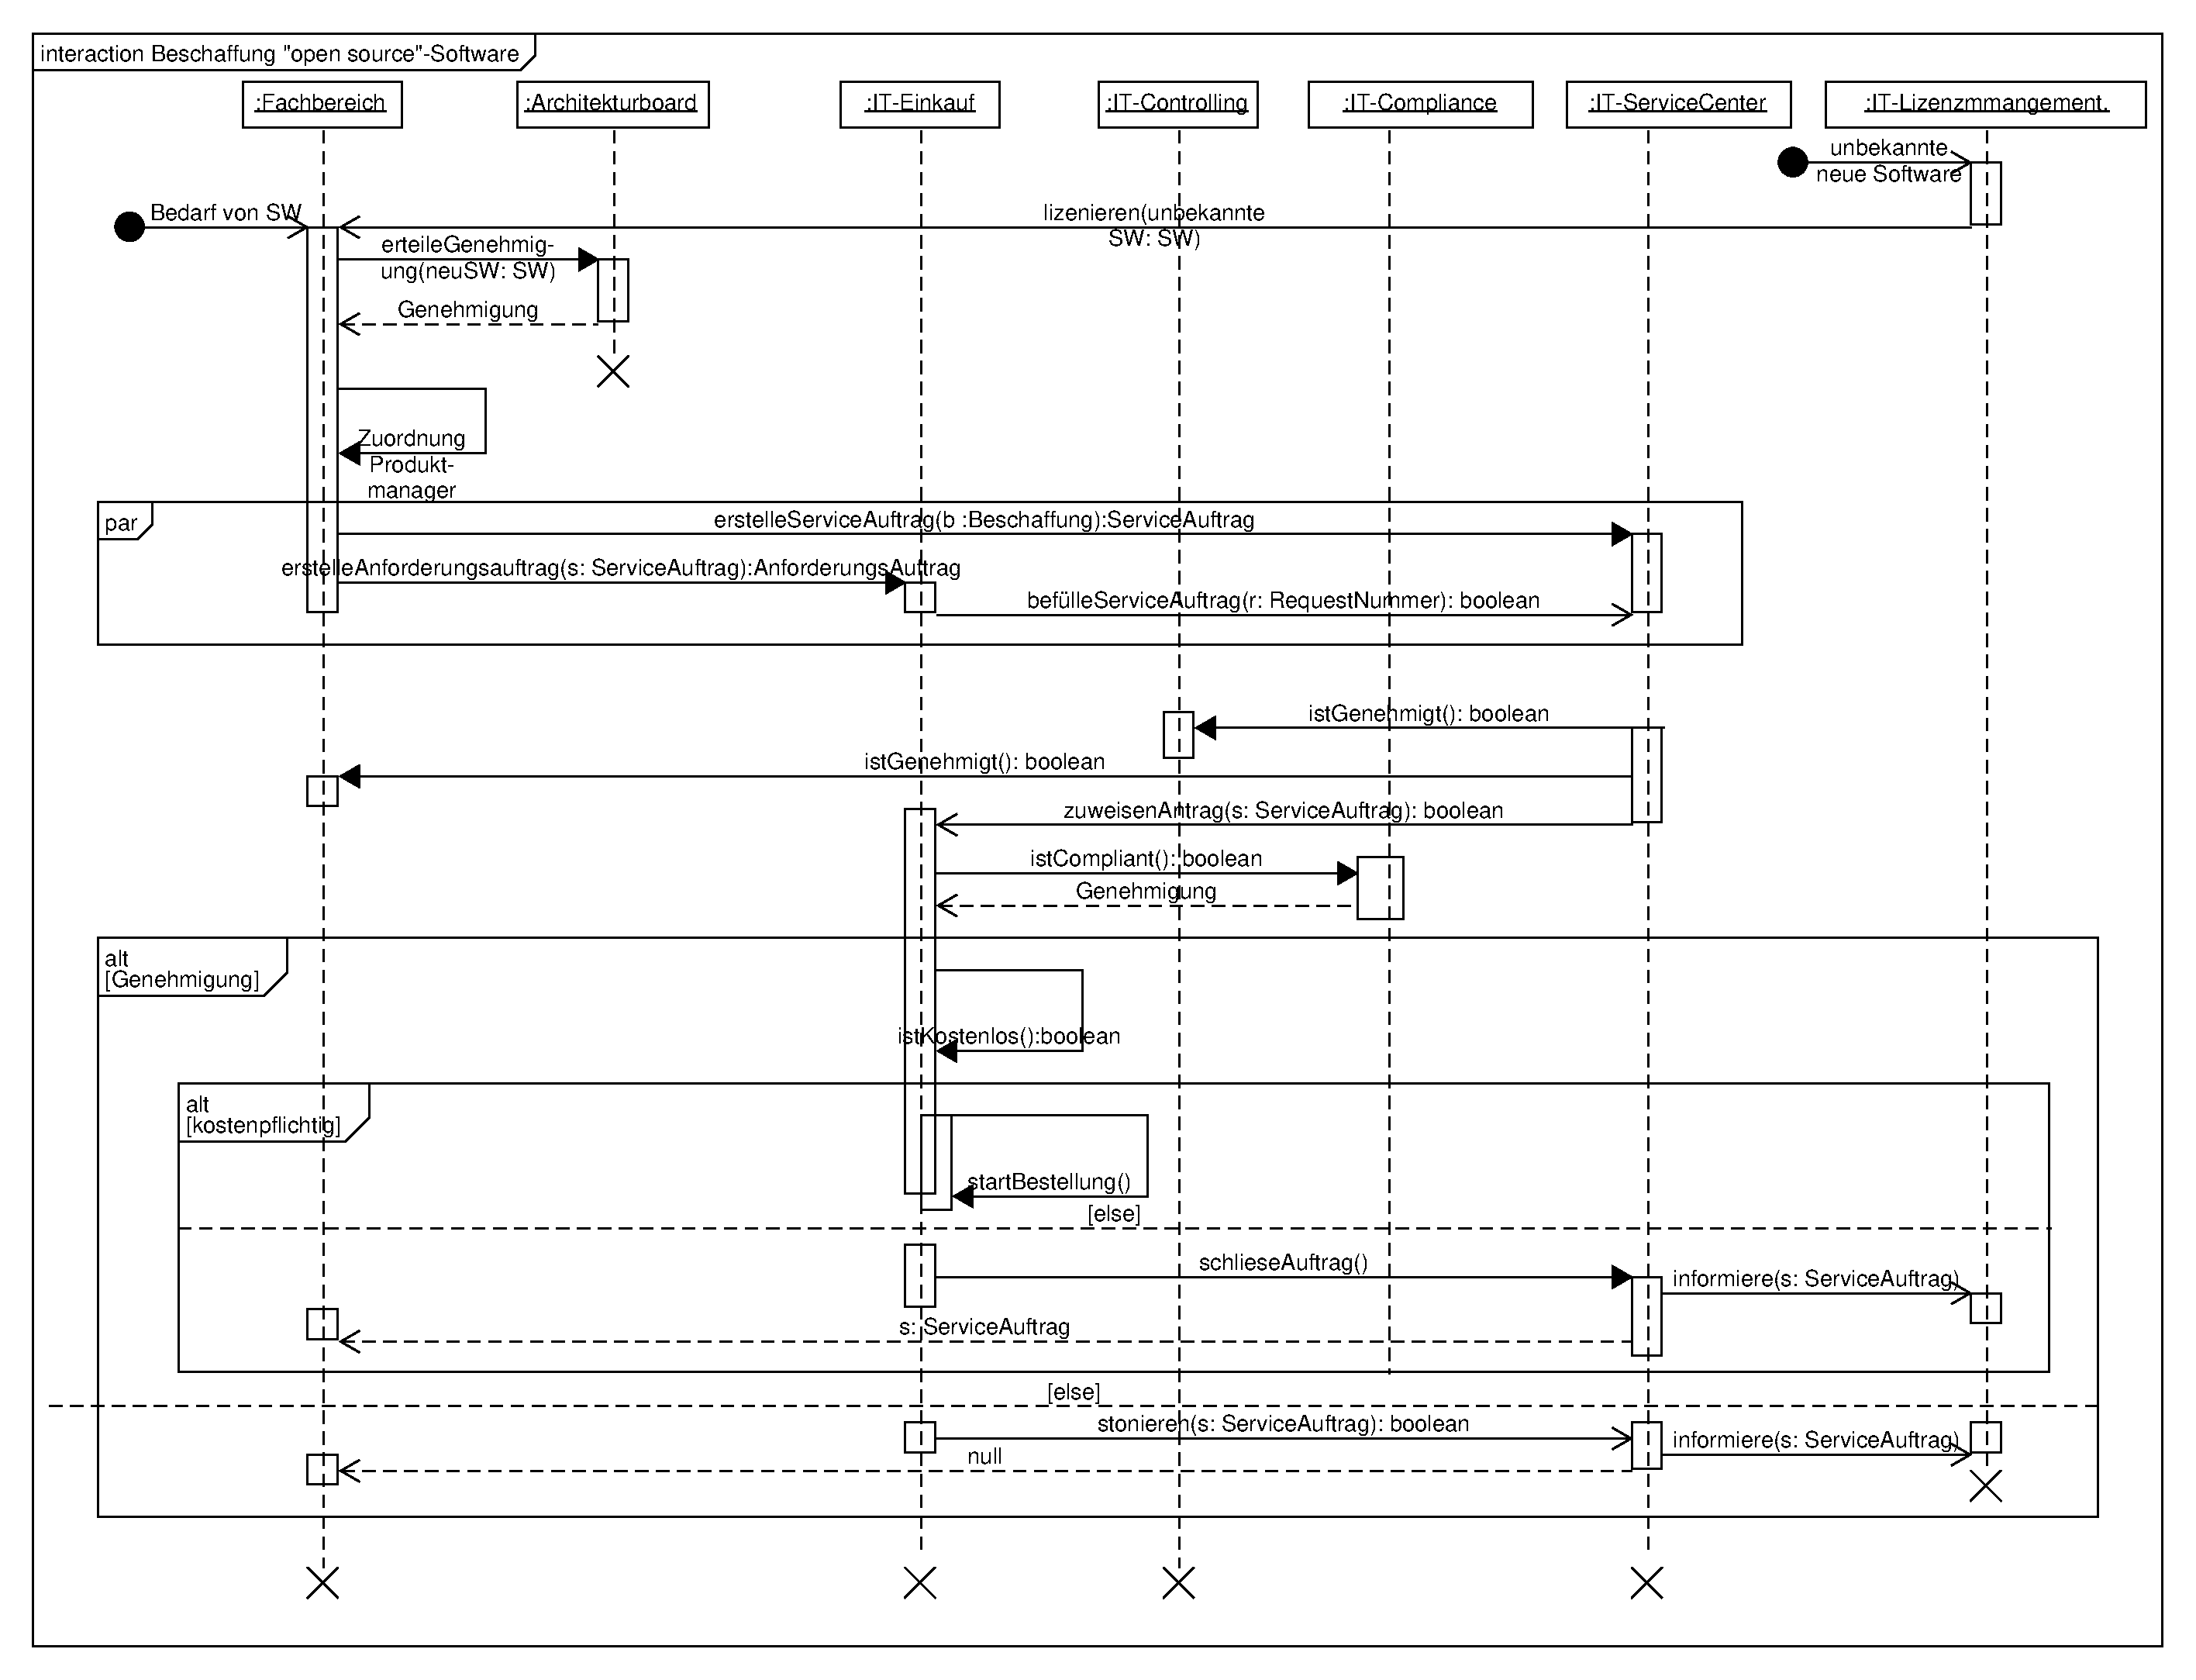
\includegraphics[scale=0.32]{img/prozessFreewareBeschaffung.pdf}
	\caption{(adaptiertes) Sequenzdiagramm zur Beschaffung von \enquote{open source}-Software}
	{\footnotesize Quelle: in Anlehnung an unternehmensinterne Prozessdokumentation \par \textit{unternehmensintern}}
	\label{abb:pFW}
\end{figure}

Die oben genannten Hürden, aus Sicht der IT-Abteilung, erfüllen nicht die Kosten-Nutzen-Konformität. Aus rechtlicher Sicht ist das ein sehr hoch zu bewertendes Risiko, da es zu unmittelbaren juristischen Konsequenzen führen kann. Deswegen nutzt die IT-Abteilung meist den rechtlichen Prozess (juristische Prüfung von Vertragsdokumenten oder Sachverhalten) da dieser nicht die oben genannten Hürden enthält. Bei diesem wird der Verwendungszweck der Software erfragt und die Lizenz dieser durch \ac{IU11} geprüft. Jedoch ist davon auszugehen, dass eine offizielle Beschaffungsanfrage bei \enquote{open source}-Software in wenigen\footnote{$ n \leq 10, n \in \mathbb{N}_{0} $, gemessen p. a.} Fällen gestellt wird. Begründet durch die Administrator-Berechtigung, die es Benutzern erlaubt ohne Restriktionen alles auf ihrem Computer zu installieren, kann keine numerische Aussage über die Dunkelziffer getroffen werden. Es bleibt nur die Hypothese der Juristen der Abteilung \ac{IU11}, die weder falsifizierbar noch validierbar ist. 
\par
Ist die Software in der \ac{AWL} implementiert, gibt es noch eine Anwendung, \textsc{Nexus Lifecycle} von \textsc{sonatype}, die auf eventuelle Schwachstellen dieser benutzten Software prüft. \textsc{Nexus Lifecycle} ist eine Hilfsanwendung, die u. a. auch von \textsc{Creditreform} verwendet wird. Das Ziel dieses Produktes ist es, die gesamte Software-\enquote{Supply Chain} kontinuierlich zu bereinigen und sicher zu halten.\autocite[vgl.][]{sonatype_inc_nexus_2020} Aus dem Prüfbericht werden dann entsprechende Maßnahmen abgeleitet. Die erste ist die Software, in der die Schwachstelle gefunden wurde, als unsicher zu markieren und danach zu sperren. Die Entwicklungsabteilung muss versuchen die Schwachstellen zu beseitigen. Problematisch ist es, wenn diese ignoriert werden. In letzter Konsequenz werden der Betrieb und die Verteilung der Anwendung gestoppt. Dies führt zu massiven Problemen in der Produktion und somit verringert sich die vertragliche, mit dem Kunden vereinbarte, Verfügbarkeit der Systeme.

\section{Konzept zur Implementierung der Sicherheitsanforderungen}

\section{Ergebnis der Forschungsfrage drei}


